\chapter{The \alphat search}

The \alphat~analysis is an hadronic search for new physics 
targeting models which are produced and which decay via the strong force.
Such strong force modes may be expected to dominate in the proton-proton collisions 
at the LHC. Exploiting an hadronic final state requires effective 
background suppression and residual background prediction. During Run 1, the \alphat~analysis 
strategy has been used for several searches for supersymmetry at
both $\sqrt{s} = 7 \TeV$ and $\sqrt{s} = 8 \TeV$ as well as a range of luminosities
\cite{alphaT1,alphaT2,alphaT3,alphaT4}. For Run 2, the selections and categorisation 
have been updated to improve the sensitivity and acceptance of the search and are detailed below.

The \alphat~analysis \emph{signal region} is defined by selecting a final state 
including jets and significant \met with no reconstructed leptons or photons
to search for new physics. To mitigate the otherwise dominant QCD multijet background, 
detailed in Section~\ref{sec:qcd-background-intro}, dedicated dimensionless variables, 
defined in Section~\ref{sec:important-variables}, are used to strongly suppress this process.
In defining the signal region, additional hadronic, kinematic and cleaning selections 
are used for further QCD and electroweak background suppression and are described in 
section~\ref{sec:had_sr}.

The determination of residual QCD multijet backgrounds as well as backgrounds with 
genuine \met~(described in Section~\ref{sec:ewk-background-intro}) relies on data driven techniques 
described in Sections ?? and ?? respectively. These data driven predictions use signal 
depleted \emph{control regions} enriched in a particular
background process (or related process). All events used in the \alphat~analysis pass
a common preselection described in Section~\ref{sec:presel}. Further selections in
these control regions closely follow those in the signal region and are detailed in 
Section~\ref{sec:cr-sel}.

As discussed in Section~\ref{sec:triggerUpgrade}, an effective trigger strategy is 
critical to ensure acceptance to models which may, for example, have relatively low
\scalht~but significant~\mht. The trigger strategy for the signal and control regions
is discussed in Section~\ref{sec:ana-trigger}.

To inclusively optimise sensitivity, the events that pass the signal region requirements 
must be categorised to allow significant signal contributions for a wide range of models. 
Several variables are used, as detailed in Section~\ref{sec:cat}, to categorise the signal region. 
The characterisation of these variables using the control
regions is shown in Section~\ref{sec:char}.

\section{Backgrounds for hadronic searches}
\subsection{The QCD multijet background}
\label{sec:qcd-background-intro}
The QCD multijet background from inelastic scattering dominates for hadronic searches at the LHC. 
The cross section for this process has been measured at $13\TeV$ as $\sim78.1mb$~\cite{inelast}. These events
are typically balanced dijet events, though higher jet multiplicities are also possible. 
Unlike the signal processes for which the $\alphat$ search is sensitive, these events contain
no true~\met. Fluctuations in detector response and reconstruction can cause a small fraction 
of the QCD events to gain significant \emph{fake}~\met. These form a dominant background as 
the total QCD cross section ($\sim78.1mb$ at $13\TeV$~\cite{inelast})
is 6 to 7 orders of magnitude larger than that of the electroweak backgrounds described in
 Section~\ref{sec:ewk-background-intro} unless suppressed. 
The main detector and reconstruction mechanisms that may introduce fake \met are summarised below:

\begin{itemize}
\item Detector inefficiencies due to regions with reduced or no response (\emph{dead cells}) can cause 
a significant proportion or all of the energy of any incident physics object to be lost. If the true event 
is balanced, losses which occur due to detector inefficiency will contain a \met~vector which points 
approximately in the $\phi$ direction of the problematic region.
\item Misreconstruction due to effects such as tracking errors, incorrect object identification and
under/over correction of jets when calibrating. This may apply to one or more objects in the event. If the 
underlying event is balanced the \met~vector will typically point in or opposite to the direction 
of the misreconstructed object in cases of under or over estimation of the energy respectively.
\item Additional energy can be added in the event due to effects including \emph{hot cells} which 
consistently record energy depositions without incident particles in the ECAL or HCAL, 
spontaneous discharges and direct particle interactions with detector
electronics or photomultipliers
\item The \emph{beam halo} of charged particles around the LHC beam, caused mainly 
by proton scattering off LHC collimators, 
may interact with muon chambers causing fake muons to be reconstructed or deposit energy 
in the calorimeters as they traverse the detector~\cite{beam_halo}. The beam halo has the largest 
effect for $\phi = 0$ and $\phi=\pi$ as the constituent particles
tend to lie within the plane of the LHC ring.
\item Imbalance nay be introduced by acceptance effects. If physics objects are excluded from the calculation
of energy sums due to thresholds in quantities such as $\pt$~or $\eta$~\met~will be introduced. These thresholds are typically 
required due to imperfect detector coverage or to remove objects reconstructed due to effects such as detector 
noise or pileup.
\end{itemize}
In addition to QCD multijet events with fake~\met discussed above, QCD scattering processes 
may produce events containing true~\met. This is due to the rare production of heavy flavour 
quarks which decay via leptons and neutrinos. These events pass hadronic selection as the leptons from 
heavy flavour decay are usually confined within the jet cone and fail isolation requirements. 
In such cases the \met~vector is typically closely aligned with the $\phi$ direction of the jet.

\subsection{Electroweak backgrounds}
\label{sec:ewk-background-intro}
%should this be in theory section?
There are several SM processes which form backgrounds for hadronic searches. These
backgrounds include \met~from neutrinos and are termed the \emph{electroweak} backgrounds. 
The dominant electroweak background processes are \wj,\ttj~and \zj. The $\alphat$
signal region, defined fully in Section~\ref{sec:had_sr}, selects purely hadronic events
containing reconstructed jets and \met. An overview of the electroweak background processes 
and the mechanisms by which they may enter into the signal region is given below. 

\subsubsection{\zj background}

The largest background process in the signal region comes from Z boson production
in association with jets (\zj) followed by decay to neutrinos, \znunu. This process is 
an \emph{irreducible} background as the neutrinos produce significant \met~in the final 
state with no associated leptons. Across the signal region, \znunu~contributes $\sim 54\%$ of 
the overall background. The decay of the Z boson to leptons, \zll~may also introduce $\met$ if 
one or both of the leptons is not reconstructed (\emph{lost}). Due to the low probability of
losing both leptons in the event, this is a sub-dominant background, comprising $\sim 0.5\%$ of the signal region.

\subsubsection{\wj background}

The production of a W boson in association with jets (\wj) where the W boson decays leptonically
(\wl) comprises $\sim 38\%$ of the overall background in the signal region. 
In such events the lepton is not reconstructed allowing them to pass hadronic selection.
This \emph{lost lepton} background may be introduced if the lepton falls out of acceptance,
fails isolation requirements or is otherwise misreconstructed. Both the lost lepton 
and the neutrino in the event may contribute to the~\met. 
% Typically, however, 
% the neutrino dominates the \met~as low $\pt$ leptons are more likely to be misreconstructed.
The branching fraction for a W decaying to an hadronically decaying $\tau$ is $\sim6\%$.
In such events the associated $\tau$ neutrino may introduce significant~\met. If the hadronic
decay products are reconstructed as a jet these events may pass the signal region selection.
To reduce this background a single isolated track is used to reject single prong decays of the 
$\tau$~($\tau{\pm}\rightarrow\pi^{\pm}+n\pi^{0}\nu$) which comprise $\sim70\%$ of the hadronic tau decays.

\subsubsection{\ttj and single top background}

The \ttj~and single top background comprise around $5\%$ and 0.5\% of the overall
background respectively. On production, the top quark will predominantly decay via the 
weak force as \twb. The W boson may then decay hadronically, producing a final state
with multiple jets or leptonically, producing a final state including a lepton and neutrino. 

The final state in an event with \ttj production will include two bottom quarks as well as multiple 
jets and/or significant \met depending on the decay. If both W bosons decay hadronically ($\sim45.7\%$ of \ttbar~decays)
up to six jets may be produced from the hadronisation of the quarks. In this case the $\met$
may be introduced via jet mismeasurement or from bottom quark decay via neutrinos. If one of the 
W bosons decays leptonically ($\sim45.8\%$ of \ttbar~decays) up to four jets may be expected
as well as~\met from the neutrino. Such events may enter hadronic selection if the lepton is lost.
Finally, if both W bosons decay leptonically ($\sim10.5\%$ of \ttbar~decays) the final state contains two 
leptons and significant \met. This mode is sub-dominant due to the low probability of losing both leptons
and lack of jets in the final state. For all decay modes the number of jets reconstructed in the event
may be increased by processes such as ISR and FSR as well as pileup.

The \alphat analysis categorises events using the number of reconstructed 
jets identified as originating from bottom quarks. The \ttbar background is particularly
enriched for $\nb \ge 2$, comprising $\sim60\%$ of the background for such events.

Single top production occurs mainly via t-channel in association with a quark, production in 
association with a W boson, or s-channel in association with a bottom quark with approximate
proportions 72.5, 24 and 3.5\% respectively. As for \ttj, the single top background is enhanced for 
categorisations with at least two reconstructed bottom quarks, rising to $\sim5\%$ of the total for
such events.

\subsubsection{Residual electroweak backgrounds}

In addition to the backgrounds discussed above, there are several processes which 
make minor contributions to the total background in the signal region (which can be enhanced
for particular categorisations). Such residual backgrounds include \ttbar production in association with a vector
boson, ($\sim0.1\%$ of the total background and $\sim4\%$ of the total background for an $\nb \ge 2$ selection); 
pair production of vector bosons, ZZ, WZ and WW ($\sim1.4\%$ of the total background); 
production of a (lost) photon in association with jets ($\sim0.7\%$ of the overall background) and
leptonic decays of the Z with two lost leptons ($\sim0.5\%$ of the overall background).

\section{Suppression of the QCD multijet background}
\label{sec:important-variables}

Predicting the QCD backgrounds presents significant challenges, discussed in Section ??, which
can introduce large uncertainty in the background estimation. A distinguishing feature
of the \alphat~analysis is the aim to mitigate this uncertainty by reducing the 
background from QCD processes to the percentage level. This is achieved using selections on
the dedicated variables \alphat, \bdphi, \mhtmet~and the forward jet veto. This section
describes how these variables distinguish QCD events from those containing true~\met
by exploiting the topologies and features of QCD events containing fake~\met. Further
event filters that specifically target events containing $\met$ introduced by
known detector problems and beam halo effects are discussed in Section~\ref{sec:event_filters}.

\subsection{\alphat}
The \alphat variable is designed to reject balanced events which gain significant~\met through
jet mismeasurement. The $\alpha$ variable was initially proposed in~\cite{Randall} and
converted into the transverse variable, $\alphat$, to allow use with hadronic collisions. The absolute
value of the $\met$ is sensitive to the detector and reconstruction effects discussed in Section~\ref{sec:qcd-background-intro} 
The \alphat variable is designed to be dimensionless such that the topology of the event is used to reject 
QCD processes, regardless of the total value of the~\met.

For a dijet event, \alphat is defined as

\begin{equation}
\label{eq:alphat}
\alphat\, =\, \frac{\Et^{{\rm j}_2}}{M_\text{T}} \, ,
\end{equation}

where $\Et^{\rm j_2}$ is the transverse energy of the 
less energetic jet and $M_\text{T}$ is the transverse
mass of the dijet system, 

\begin{equation}
  \label{eq:mt}
  M_\text{T}\, = \,\sqrt{ \left( \sum_{i=1}^2 \Et^{{\rm j}_i}
    \right)^2 - \left( \sum_{i=1}^2 p_x^{{\rm j}_i} \right)^2 - \left(
      \sum_{i=1}^2 p_y^{{\rm j}_i} \right)^2} \, .
\end{equation}

where $\Et^{{\rm j}_i}$ is the transverse energy of jet ${\rm j}_i$ (
$\Et^{{\rm j}_i} = E^{{\rm j}_i}\sin\theta^{{\rm j}_i}$), and
$p_x^{{\rm j}_i}$ and $p_y^{{\rm j}_i}$ are the $x$ and $y$ components
of the transverse momentum of the jet. 

For events with three or more jets a pseudo-dijet system is defined 
where all possible vectorial sums of the jets in the event into two
pseudo-jets are considered. The combination into pseudo-jets 
with the smallest difference in transverse energy, $\Delta E_T$, is chosen
as the most balanced configuration and used to define \alphat. The $M_\text{T}$ for 
the event is insensitive to the clustering and is given by

\begin{equation}
  \label{eq:mt_njet}
  M_\text{T}\, = \,\sqrt{ \left( \sum_{i=1}^2 \Et^{{\rm{j}}_i}
    \right) - \mht^2}.
\end{equation}

where the sum is over all jets in the event. The sub-leading psuedo jet energy,$E_{\textrm{T}}^{j'_2}$, 
is given by

\begin{equation}
E_{\textrm{T}}^{j'_2} = \frac{\sum_{i} E_{\textrm{T}}^{j_i} - \Delta E_{\textrm{T}}}{2}.
\end{equation}

The definition of \alphat for any number of jets is therefore

\begin{equation}
  \label{eq:alphat2}
   \alphat = \frac{\sum_{i} E_{\textrm{T}}^{j_i} - \Delta E_{\textrm{T}}}{2\sqrt{\left(\sum_{i} E_{\textrm{T}}^{j_i}\right)^2 - \mht^2}}.
\end{equation}

Most jets in the event contain significant boost such that $E_{\textrm{T}} \sim \pt$. The \alphat 
definition can be approximated in this case by

\begin{equation}
  \label{eq:alphat3}
   \alphat \approx \frac{\scalht - \Delta H_{\textrm{T}}}{2\sqrt{\scalht^2 - \mht^2}}.
\end{equation}

\begin{figure}
\centering
    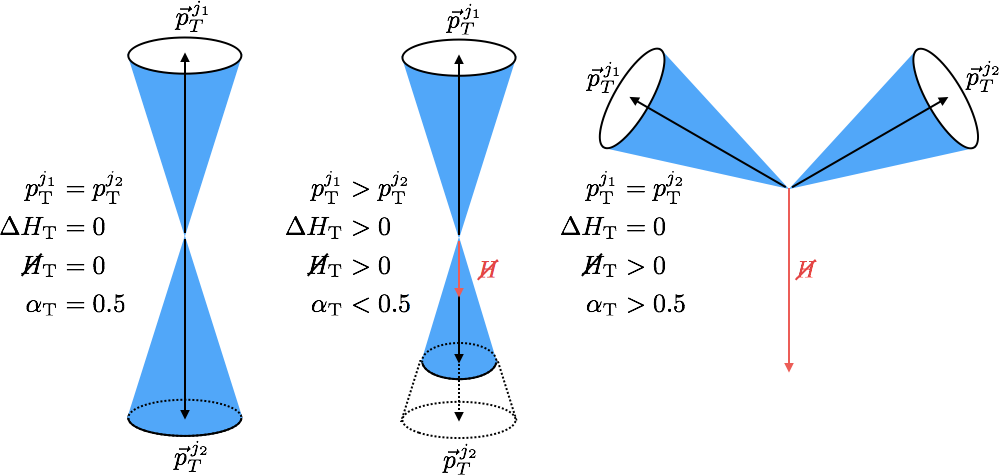
\includegraphics[width=0.8\textwidth]{./Figures/alphat/alphat_cartoon}
  \caption{\label{fig:alphat_cartoon} The \alphat~variable inputs and values for three types of event: balanced and well measured jets (left), balanced jets with
  a mismeasured jet (middle) and well measured jets recoiling against true~\met (right). The solid cones signify the reconstructed jet momentum while the 
  dashed cones represent the true momentum. The calculation of \alphat~is described in the text.} 
\end{figure}
where $\Delta H_{\textrm{T}}$ is the difference in \pt~of the pseudo jets.

To illustrate the mechanism by which the \alphat~variable rejects $\met$ from mismeasured or lost jets,
consider a dijet event as shown in Figure~\ref{fig:alphat_cartoon}. Three possible event topologies are shown: 
a perfectly balanced event (left), a perfectly balanced event with a mismeasured jet (middle) and an event containing true \met~(right).
In a balanced dijet event without mismeasurement, $Delta E_T = \mht = 0$ and the 
value of \alphat will be 0.5. If one of the jets is under or over measured for an otherwise balanced dijet
event, $\Delta H_{\textrm{T}} = \mht$ and Equation~\ref{eq:alphat3} can be written as 

\begin{equation}
  \label{eq:alphat4}
   \alphat \approx \sqrt{\left(\frac{\scalht^2 - \mht^2}{2\scalht^2 + \mht^2}\right)} < 0.5.
\end{equation}

Conversely, if an event contains true $\met$ and the jets are recoiling against significant~\met 
(which is not aligned with one of the jets in the event), as shown on the right of 
Figure~\ref{fig:alphat_cartoon}, $\alphat > 0.5$. 

In the general case of two or more jets, for events containing \met~from mismeasurement or 
neutrinos produced in heavy flavour decays the values of $\Delta E_{\textrm{T}}$ and \mht~are highly correlated, leading
to values of $\alphat <= 0.5$. This correlation is much weaker in the case of pair produced, 
R-parity conserving SUSY events where each decay chain ends in the 
undetected LSP and for SM processes containing genuine \met, allowing $\alphat > 0.5$.

\begin{figure}[!htb]
  \centering
    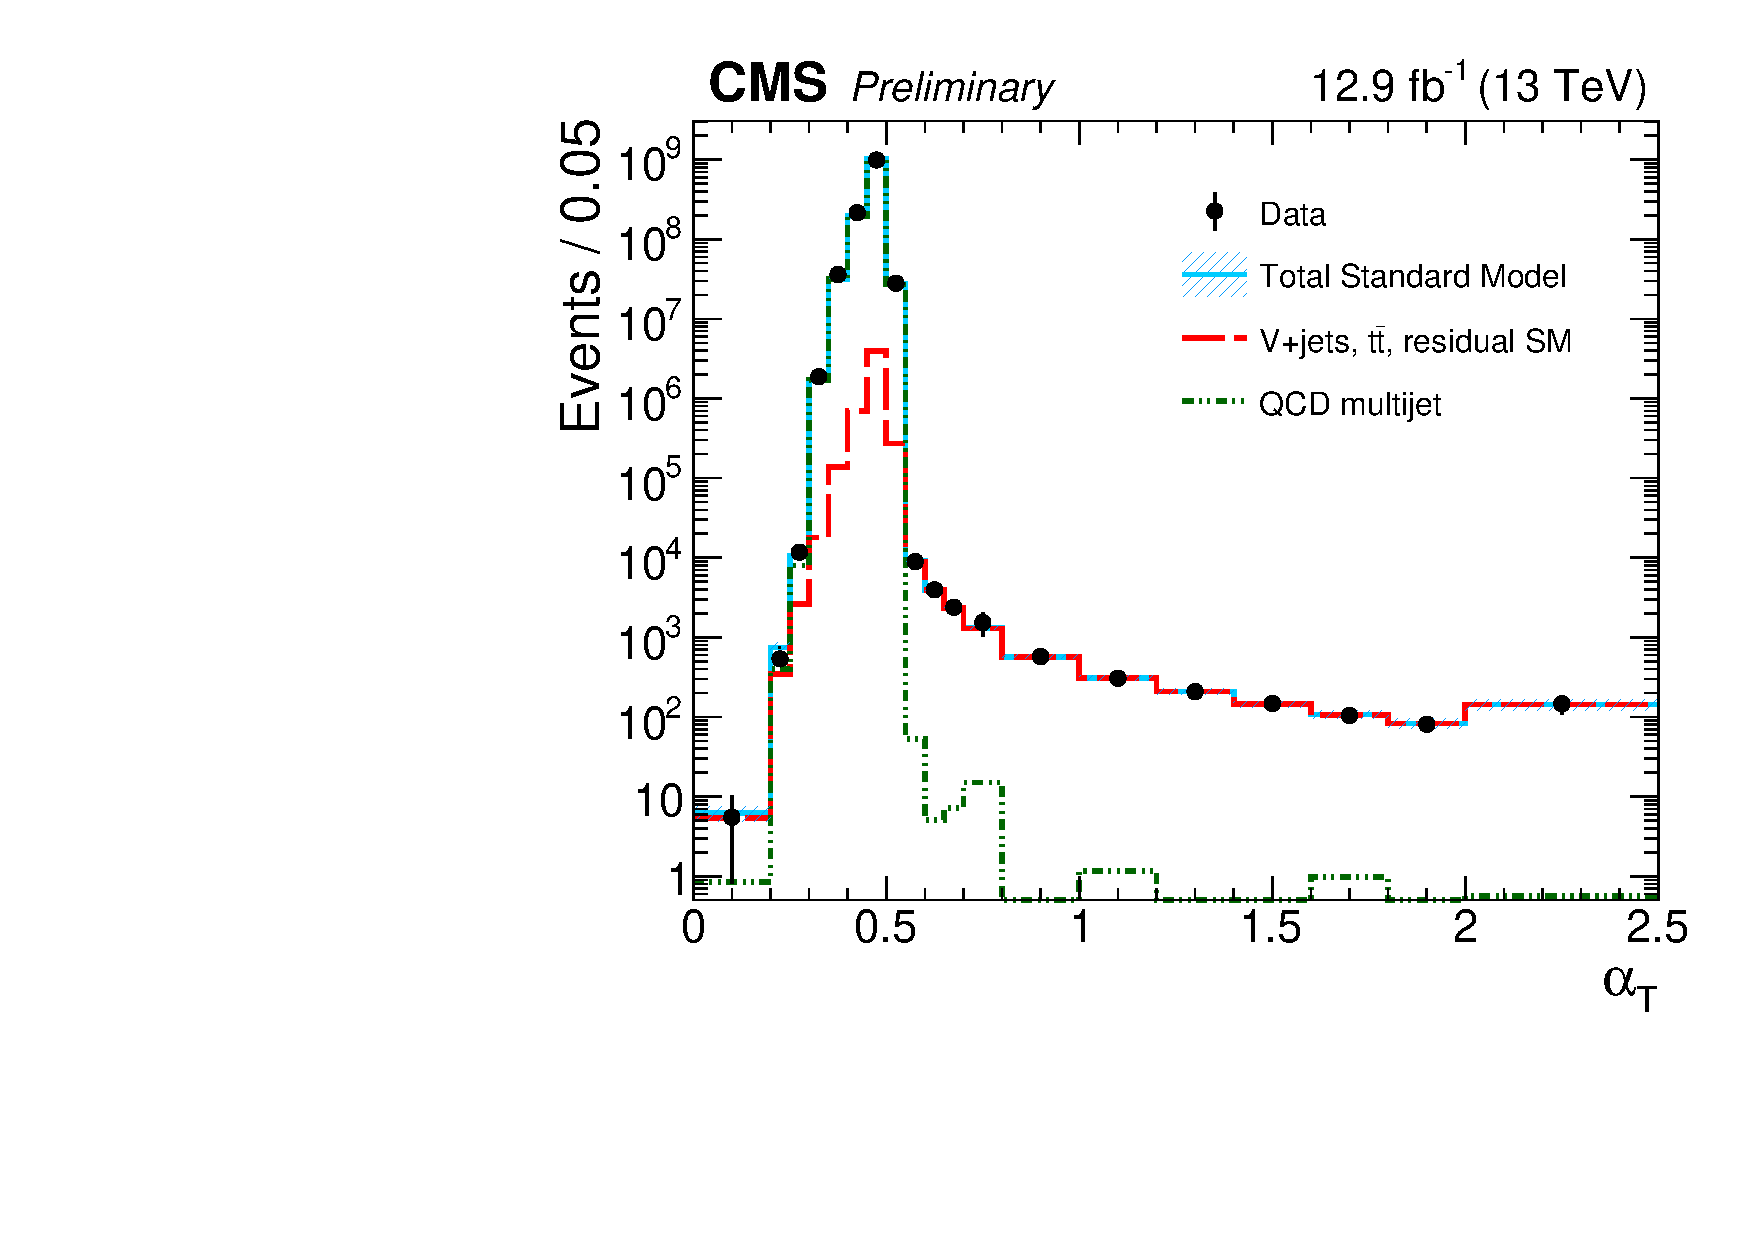
\includegraphics[width=0.49\textwidth]{./Figures/alphat/alphat_data.pdf}
  \caption{
    The \alphat distribution observed in data compared to simulation. 
    The statistical uncertainties for the multijet and SM
    expectations are represented by the hatched areas. 
    The final bin of each distribution contains the overflow events. The events below $\alphat= 0.55$ use unbiased triggers with
    a loose preselection while events above $\alphat = 0.55$ use the signal region triggers and selection.
    }
  \label{fig:alphat-data}
\end{figure}

The \alphat~distribution is shown in Figure~\ref{fig:alphat-data}. The region of $\alphat < 0.5$ is dominated by
QCD multijet events which sharply drops as \alphat~increases above 0.5. Multijet events with
very rare large stochastic fluctuations in the measured jet energies can lead
to values of \alphat~above 0.5. \footnote{QCD multijet events may also have \alphat values larger than 0.5 if the 
\pt of one or more jets is sufficiently different from $E_T$, breaking the assumption used for Equation~\ref{eq:alphat4}. 
However, this is found to have $< 1\%$ effect on the number of QCD multijet events passing $\alphat > 0.5$.}
The \alphat~distribution becomes more sharply peaked with increasing \scalht~in the event as mismeasurements are larger
 for lower jet \pt. Significantly larger values of \alphat~for QCD multijet events can also be caused by 
hot cells or acceptance effects. These are mitigated by the other discriminating variables 
discussed below and dedicated event filters. 

Unlike the QCD processes, the electroweak backgrounds have a long tail in
values of $\alphat$ greater than 0.5. The \alphat~variable allows a powerful discrimination 
between the otherwise dominant QCD background and processes with \met~well
separated from the jets.


\subsection{\bdphi}
\begin{figure}
\centering
    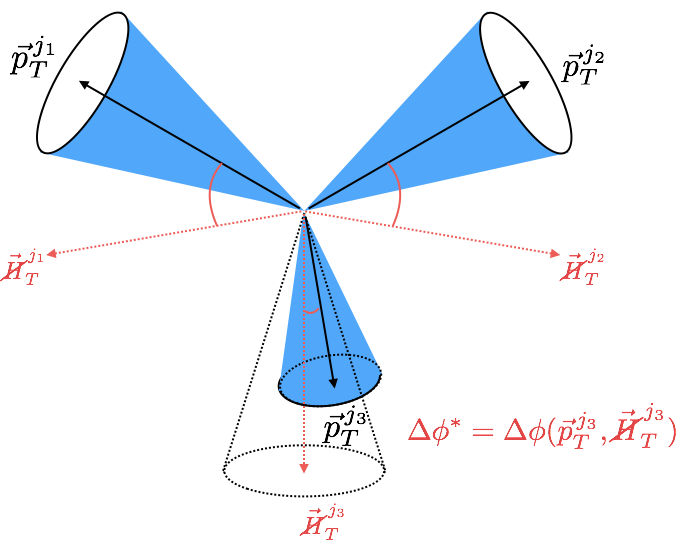
\includegraphics[width=0.8\textwidth]{./Figures/alphat/bdphi_cartoon}
  \caption{\label{fig:bdphi_cartoon} The \bdphi~variable inputs and values for a mismeasured balanced three jet event.
  The third jet minimises the $\Delta \phi_i$ and is used to calculate \bdphi~as described in the text.}
\end{figure}
The \bdphi~variable is an additional topological variable designed to mitigate contamination
from mismeasured events (from reconstruction and instrumental issues) and semi-leptonic 
heavy flavour decays. The variable is defined as follows:
\begin{itemize}
\item Each jet in the event is considered in turn as the probe jet, $j_i$.
\item The \mhtvec~is recalculated with the probe jet removed, $\mhtvec^{j_i}$.
\item The azimuthal separation of the probe jet and $\mhtvec^{j_i}$ is calculated, $\Delta \phi_i$
\item The \bdphi~is calculated as the minimal $\Delta \phi_i$ over all jets in the event,
\begin{equation}
\label{equ:bdphi}
\bdphi = \underset{\forall\, i\, \in \left[1,\nj\right]}{min} \Delta \phi_i.
\end{equation}
\end{itemize}

If the \bdphi~value is close to the jet cone size, the jet which minimizes $\Delta \phi_i$ (\jbdphi)~is likely 
to be mismeasured or contain~\met~from a leptonic decay of a heavy flavour quark. The \bdphi~variable is insensitive to
the~\pt of \jbdphi~and rejects events containing a jet whose \pt~is either over or under measured.
The jets in the electroweak background processes and signal models typically recoil against the
\met~implying larger values of \bdphi. The calculation of \bdphi~for a mismeasured balanced 
event containing three jets is shown in Figure~\ref{fig:bdphi_cartoon}.
In the \alphat~analysis a threshold of 0.5 is used to reject QCD multijet events.

The \bdphi~variable can be compared to the nominal minimal $\Delta \phi$~between
the \mht~and the lead four jets in the event used by many hadronic analyses, \dphimhtj.
The advantages of \bdphi~include sensitivity to mismeasurement of any jet in the 
event (not merely the lead four), sensitivity to both under and over measurement
of jet energies (\dphimhtj~does not provide rejection of events with an over-measured jet)
and insensitivity to the \pt~of the jet which is mismeasured. Given these advantages, 
the \bdphi~variable can provide an order of magnitude better rejection of QCD for the 
same signal efficiency for a SUSY model containing significant \met~and hadronic activity.

\begin{figure}[!htb]
  \centering
    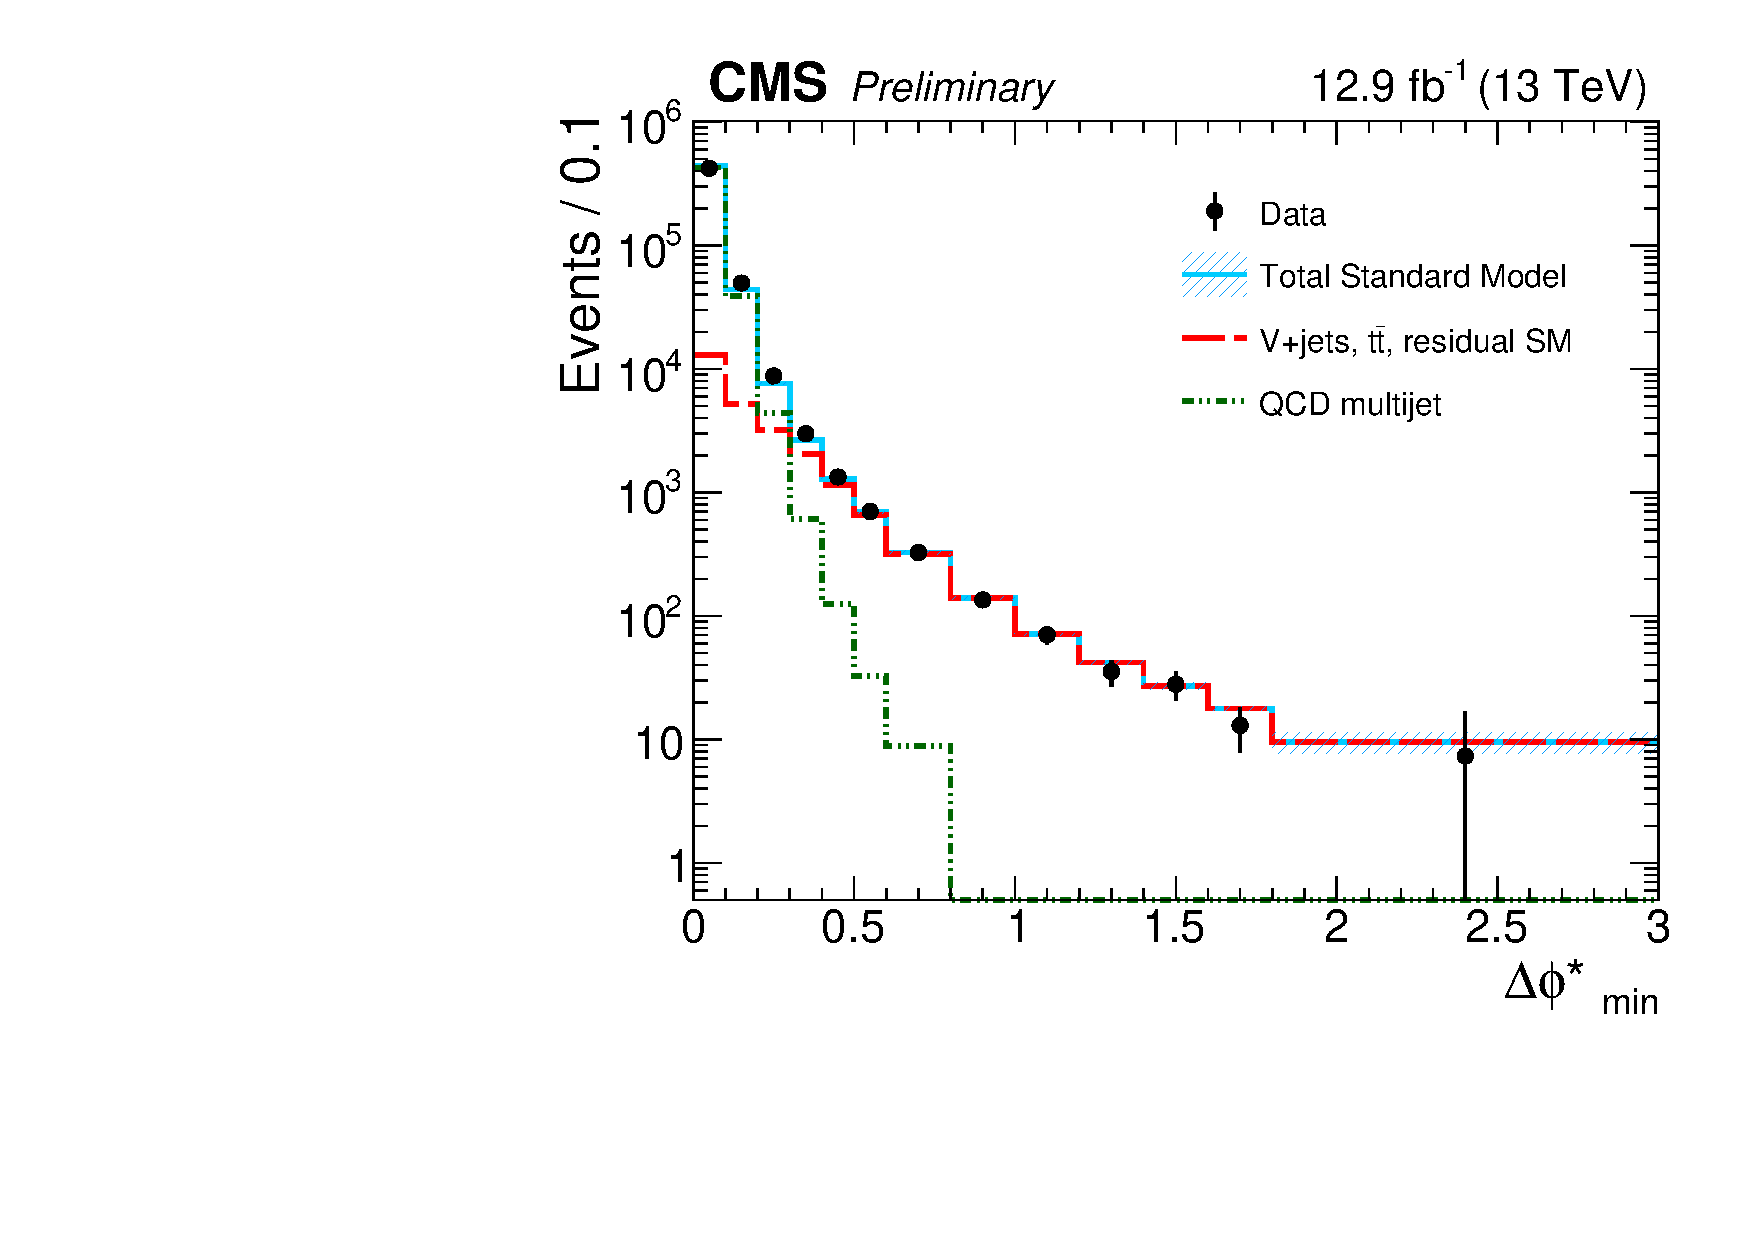
\includegraphics[width=0.49\textwidth]{./Figures/alphat/bdphi_data.pdf}
  \caption{
    The \bdphi~distribution observed in data compared to simulation for a selection $\scalht > 800\GeV$.
    The statistical uncertainties for the multijet and SM expectations are represented by the hatched areas. 
    }
  \label{fig:bdphi-data}
\end{figure}

The distribution of \bdphi~in data and simulation for $\scalht > 800\GeV$ is shown in Figure~\ref{fig:bdphi-data}.
The QCD multijet background is seen to decrease by around five orders of magnitude as \bdphi increases
to 0.5. In Figure~\ref{fig:bdphi-data} the electroweak background processes
can be seed to have long tails up to $\bdphi = \pi$.

\subsection{\mhtmet}
The \mhtmet~cleaning cut is designed to reduce the contamination from balanced events
due to acceptance effects from kinematic and pseudorapidity thresholds, 
severe jet mismeasurement and particles not clustered into jets. The PF \met~includes
all PF candidates and so the contamination from such events may be mitigated 
using a maximal threshold on the ratio of the \mht~to the \met.
\subsection{Forward jet veto}
\label{sec:fwd_jet_veto}
The $\mht$ variable is made using jets with $\etaabs < 2.4$. Jets in the forward pseudorapidity 
region will may introduce $\mht$. A veto on any jet in the forward region with $p_T > 40\GeV$
is used to reject such events. 



\section{Preselection}
\ref{sec:presel}
The objects described in Section~\ref{sec:phys-obj} are used to define a common kinematic 
preselection for the signal and control regions used in the $\alphat$ analysis. 
The kinematic selections as well as event filters and vetoes targeting
known instrumental, reconstruction and beam effects are described in this Section.

\subsection{Kinematic selections}
The minimal requirements on the energy sums for both the signal and control regions are
$\scalht > 200\GeV$ and $\mht > 200\GeV$. In addition, at least one jet satisfying the 
requirements detailed in Table~\ref{tab:kine-sel} is required. These selections are 
designed by considering trigger efficiency constraints while maximising acceptance for
signal models with small mass splittings.
\subsection{Event filters}
\label{sec:event_filters}
Event filters reject events contaminated by detector or reconstruction effects
which can cause significant~\met. Such effects may not be known when the 
background simulations are produced or can be difficult to simulate. Therefore,
dedicated filters are used to remove such events in the data. These \met filters are summarised below,

\begin{itemize}
\item The \emph{HBHE noise and isolation filters} reject energy spikes in the HCAL caused by noise from sources 
including direct particle interactions with HCAL instrumentation.
\item The \emph{EE bad supercluster filter} removes events containing \TeV scale energy spikes from anomalous
pulses in the EE.
\item The \emph{CSC beam halo filter} uses the CSC to measure halo muons and reject events containing 
significant contamination from the beam halo.
\item The \emph{ECAL trigger primitive filter} rejects events where significant energy is deposited in dead cell regions.
\item The \emph{Primary vertex filter} requires at least one well reconstructed vertex which ensures collisions have occurred
rather than an event triggered and reconstructed from detector noise.
\item The \emph{bad muon and bad charged hadron filters} reject events containing poorly reconstructed muons reconstructed as 
a muon or PF charged hadron respectively.
\end{itemize}

\begin{figure}
\centering
    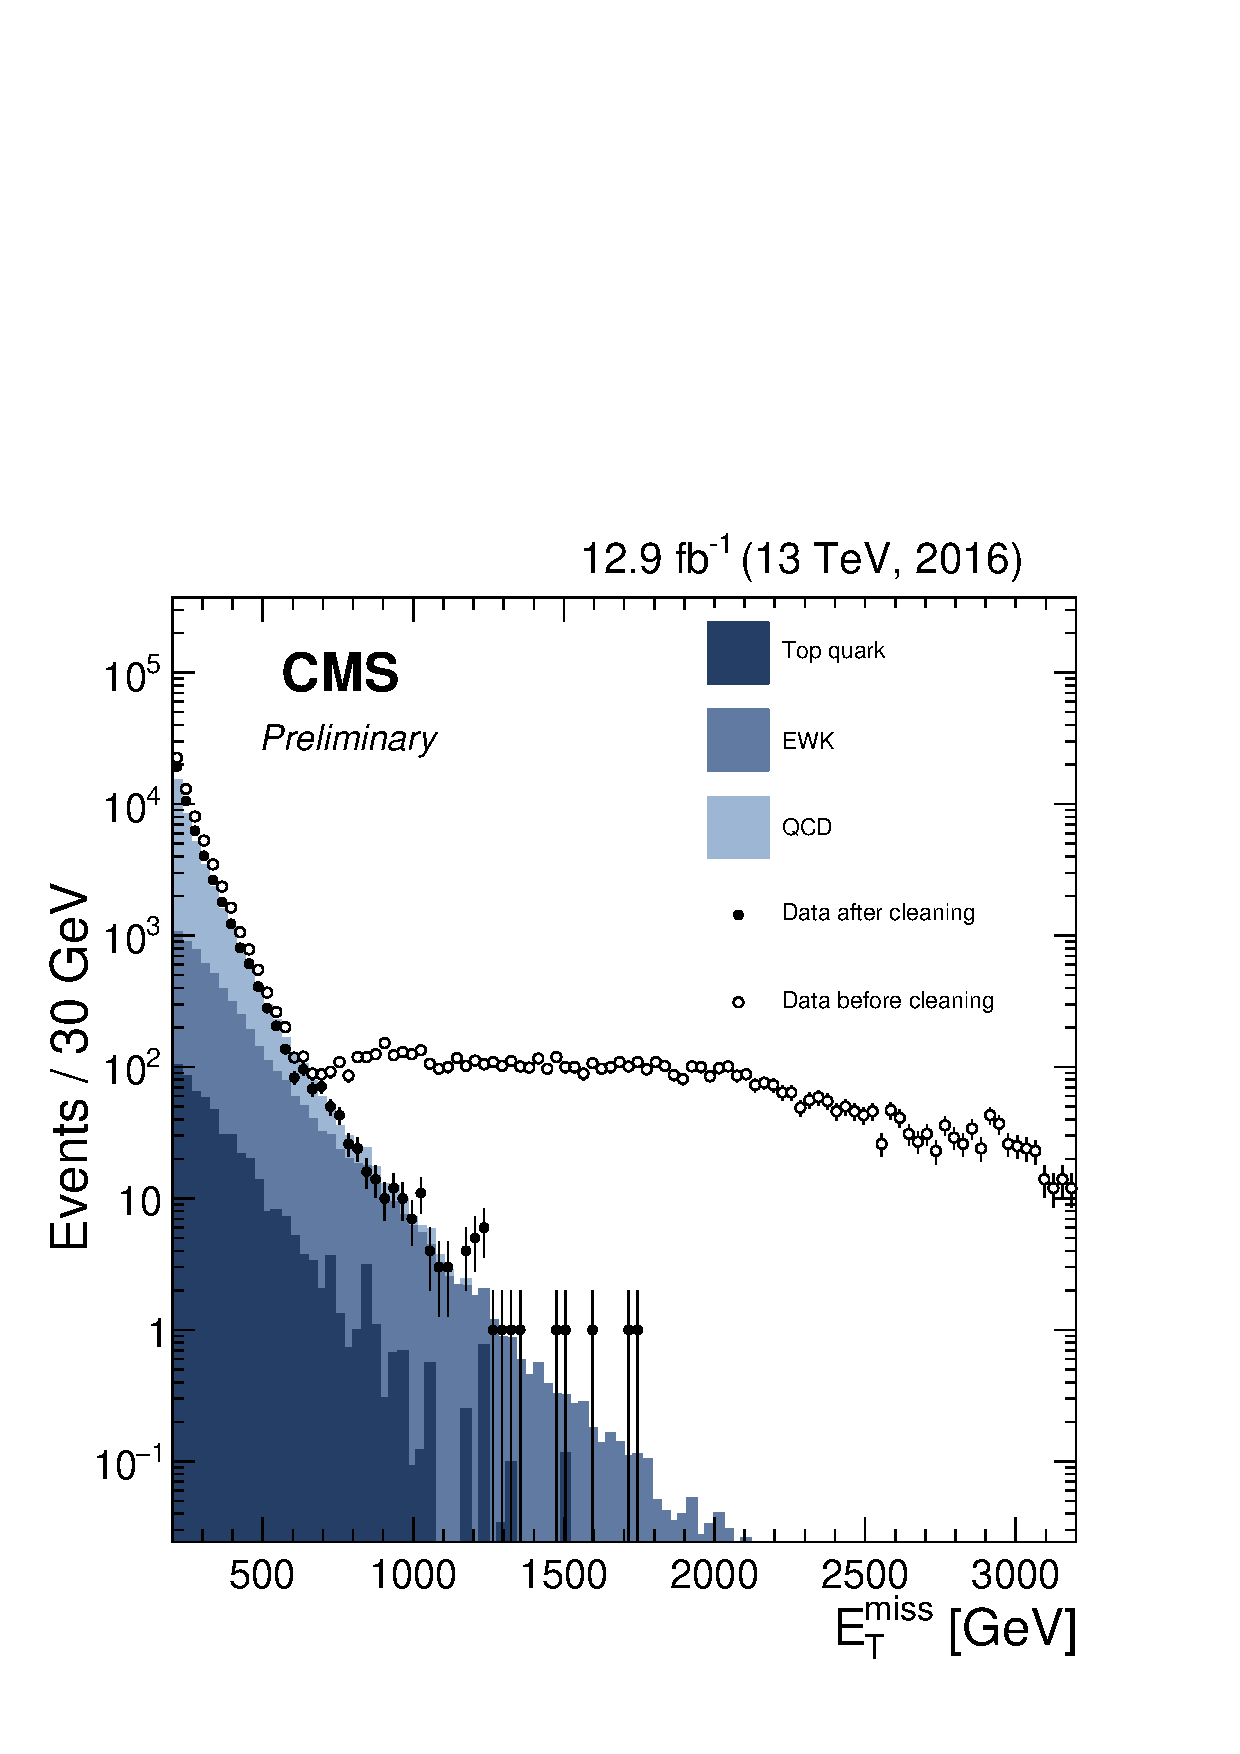
\includegraphics[width=0.8\textwidth]{./Figures/alphat/met_clean}
  \caption{\label{fig:met_filter} The $\met$~filters remove the long tail in the reconstructed \met~caused by detector, reconstruction
  and beam effects in the data~\cite{met_fig}.} 
\end{figure}
The performance of the \met~filters for the reconstructed \met~in the data is shown in Figure~\ref{met_fig}. The long tail caused by
the effects in data discussed above is mitigated by the filters. In addition to the \met~filters, 
additional vetoes are used by the \alphat~analysis to reject events affected by misreconstruction and residual beam halo. These are
\begin{itemize}
\item A \emph{leading jet charged hadron energy fraction (CHEF) veto} which rejects events 
contaminated by beam halo energy deposits which pass the CSC beam halo filter. The lead jet 
in the event is required to satisfy CHEF > 0.1.
\item The \emph{odd jet veto} rejects any event containing a jet which fails the 
requirements in Table~\ref{tab:loose-jet-id}. These are often caused by noise or misreconstruction.
\item The \emph{forward jet veto}, described in Section~\ref{sec:fwd_jet_veto}, rejects events containing jets which fall out of acceptance but
are reconstructed in the forward region. 
\end{itemize}
%%MAYBE ADD PLOTS HERE TO MOTIVATE?

\section{Analysis selections}
The common preselections are applied for all events used by the \alphat~analysis. The events 
passing these selections may then fall into the signal region or the hadronic,
\gj, \mj or \mmj control region. These regions are exclusive such that no
event may be double counted and the selections for each are summarised below.

\subsection{Hadronic signal region}
\label{sec:had_sr}
Events in the signal region are categorised (see Section~\ref{sec:cat}) and used
to search for hadronic signatures of new physics. Selections are made to suppress the QCD multijet
background and reducible electroweak backgrounds.
\subsubsection{QCD background suppression}
\label{sec:qcd_sup}
The QCD multijet background is suppressed using thresholds on 
the \alphat, \bdphi~and \mhtmet~variables and event filters.
A \scalht dependant threshold is used to account for the broadening \alphat distribution
for lower \scalht values. These thresholds must also be efficient considering
the trigger requirements and are shown in Table~\ref{tab:alphat-thresholds}. The highest threshold 
of 0.65 is used for $200\GeV < \scalht < 300\GeV$ while there is no \alphat~
requirement for $\scalht > 900\GeV$, for which region a pure \scalht~trigger is used.
At least two jets are required to define~\alphat and therefore no threshold is used
in events containing only one jet (monojet).

\begin{table}[h!]
  \caption{\alphat thresholds versus
    lower bound of \scalht bin. For all \scalht bins satisfying $\scalht >
    900\gev$, no \alphat cut is applied. No \alphat requirement is
    imposed in the monojet bins.}
  \label{tab:alphat-thresholds}
  \centering
  \footnotesize
  \begin{tabular}{ lccccccccc }
    \hline
    \hline
    \scalht            & 200       & 250       & 300       & 350       & 400       & 500       & 600 &  $>$900    \\
    \hline                                                                                     
    \alphat threshold  & 0.65      & 0.60      & 0.55      & 0.53      & 0.52      & 0.52      & 0.52 & --    \\
    \hline
    \hline
  \end{tabular}
\end{table}

A \bdphi~threshold of 0.5 is used for all events passing signal region selection.
This value is motivated by the jet cone size of 0.4 and desired level of 
QCD suppression. For monojet events the \bdphi variable is defined including jets with 
$\pt > 20 \GeV$, $\bdphi_{20}$. If there are no such jets no threshold on \bdphi is used.
In such cases the QCD contamination is low due to the highly asymmetric event topology required.

Finally, an $\mhtmet < 1.25$ requirement rejects events containing 
\mht~due to energy present in the event which is not clustered into jets. 
The values of the thresholds on \alphat, \bdphi~and \mhtmet~provide the desired 
level of QCD multijet contamination, measured in data, of < 10\% 
as measured in data (see Section ??).
\subsubsection{Electroweak background suppression}

The electroweak backgrounds containing \met~from final states including
leptons (including \wl~and \tlb) can be suppressed by vetoing leptons. 
An additional veto on photons ensures a purely hadronic final state.
Isolated tracks are used to identify W boson decays and single prong 
decays of the $tau$. An events is vetoes if it contains at least one isolated track.
\subsection{Control regions}
\label{sec:cr-sel}
The control regions are used to predict both the residual QCD multijet
and electroweak backgrounds. Each of the control regions is enriched 
in the background sample(s) predicted by that control region or a related 
process. The selections used are described in this section and are designed to 
be as close to the signal region selections as possible 
while ensuring a large sample of events enriched in the relevant process. 
\subsubsection{Hadronic control regions}
The hadronic control regions are used to determine the level of QCD contamination
remaining in the signal region. These are defined by inverting the selection on the 
discriminating variables described in Section~\ref{sec:important-variables} to give a data sample 
dominated by events from QCD processes. Any event containing a reconstructed photon or lepton is vetoed.
\subsubsection{Photon control region}
The \gj~control region is used to predict the \znunu~background in the signal region.
One photon satisfying the requirements in Table~\ref{tab:kine-sel} is required in the 
event and events containing leptons are vetoed. The energy sums are then calculated without this photon. To reduce the reliance on simulation, 
all signal region selections are made except for those on the \bdphi~and \alphat variables.
These requirements are removed to enhance the statistics in the control region sample 
for predicting the \znunu~background. To ensure the photon is not affected by hadronic
activity, any events with a jet satisfying $\Delta R(j,\gamma) < 1$ are vetoed. Finally,
the $\mht > 200 \GeV$ threshold in both signal and control helps ensure the Z is sufficiently
boosted such that its mass does not bias the prediction from the \gj control region. 
\subsubsection{Muon control regions}
The muons used for the muon control regions are defined as detailed in
Table~\ref{tab:kine-sel}. Energy sums are defined without including the muon 
and all selections except for those on the \bdphi~and \alphat~variables are used.
Events are vetoed if $\Delta R(j,\mu) < 0.5$ for all jets and muons in the event to
ensure no hadronic activity affects the muon(s). Events are also rejected if they 
contain an electron or photon.

The \mj~control region is used to predict the lost lepton background from 
a sample rich in \wj~and \ttbar~processes. A single muon is required and a selection used on the transverse mass variable,
$\mt(\mu,\met) = \sqrt(2E^{\mu}_{T}\met(1-cos_{\Delta\phi_{\mu,\met}}))$,
of $\mt(\mu,\met) = 2E^{\mu}_{T}\met(1-cosm_{mu} < 125\GeV$ to enrich the sample with \wj~and to ensure signal model depletion.

The \mmj~control region is used along with the \gj~control region to predict the \znunu~background
using a sample rich in the \zmmj~process. Exactly two oppositely charged muons are required with
an invariant mass within 25\GeV of the mass of the Z boson, $|M_{\mu_1,\mu_2} - m_Z| < 25\GeV$.
of $\mt(\mu,\met) < 125\GeV$ to enrich the sample with \wj~and to ensure signal model depletion.

% \subsection{summary}




The L1 trigger seeds used 
\subsection{Control regions}
%Should this be earlier?

\section{Categorisation}
\label{sec:cat}
In order to maintain sensitivity to a wide range of signal models events are categorised using
several discriminating variables Each \emph{bin} may be sensitive to signal models with different 
signatures. The categorisation and targeted signal features are described in this section.

The \alphat~analysis uses a categorisation in \njet, \nb~and \scalht~for both 
the signal and control regions. Each signal region category is therefore predicted using an identical 
selection in these variables for the control region. The categorisations are determined through requirements of sufficient
control region statistics to predict each \njet, \nb and \scalht bin as detailed below. The signal region is 
further categorised according to~\mht. 

\subsection{Categorisation in \njet}

The \alphat analysis categorises events into three topologies, \emph{monojet},\emph{asymmetric} 
and \emph{symmetric}, using selections on the second jet~\pt. For all topologies, the leading
jet must satisfy $\pt^{j_1} > 100 \GeV$.  The monojet topology vetoes events containing a second 
jet with $\pt^{j_2} > 40 \GeV$ and is designed to target generic DM 
and compressed SUSY models. No jets are produced in s-channel and t-channel production of DM
while for compressed supersymmetric models, the LSP carries the majority of the energy from 
the heavy sparticle decay, meaning any jets produced in the decay are soft (small values of \pt). 
These events may come into acceptance if one of the incoming/outgoing partons radiate a jet, initial/final state
radiation (ISR/FSR), which is reconstructed. The monojet topology also rejects backgrounds from 
\ttbar which tends to have high \njet multiplicities. The asymmetric topology selects events 
containing a second jet with $40 \GeV < \pt^{j_2} < 100 \GeV$.
Compressed SUSY models whose decay products are soft but can be reconstructed and models
containing multiple ISR/FSR jets are targeted. Finally, the symmetric topology requires  
$\pt^{j_2} > 100 \GeV$ and targets more generic supersymmetric models with large mass splittings 
for which the decay products carry a large energy.

The jet multiplicity varies widely depending on the signal model and background process.
Supersymmetric signal models which predominantly involve the production light quarks and/or models 
with small mass splittings between the coloured particles and the LSP tend to produce 
a small number of jets with significant energy. Conversely, models of gluino or stop production
have larger jet multiplicities. The backgrounds are also largely \njet~dependant as 
\ttbar~decays typically produce high multiplicities while decays of vector boson backgrounds
produce low multiplicities. The events with a symmetric topology are therefore categorised according
to $\njet = 2,3,4,5,\ge6$.

\subsection{Categorisation in \nb}

A categorisation on \nb~improves sensitivity to models containing heavy flavour squarks and gluino
decays to heavy flavour quarks. Such models are favoured due to the naturalness of the
inverted mass hierarchy and can produce from 2 to 4 bottom quarks depending on the decay.
Events are categorised as $\njet = 0,1,2,3,\ge4$. The dominant background for events 
with more than one b jet comes from the \ttbar process. The misidentification of 
jets from light flavoured quarks as b jets increases the background rate for a high $\nb$ selection.

\subsection{Categorisation in \scalht}

The \scalht produced in an event provides a measure of the mass scale of 
new physics models. This will be dependant on the mass splitting between
the heavy sparticle and LSP in the model which determines the energy
provided to the visible decay products. The control regions are binned
as in~\ref{tab:ht-binning} In the signal region the \scalht categorisation depends 
on the jet category. The finest \scalht regions are shown in Table~\ref{tab:ht-binning}
These are merged from above depending on the requirement of at least one control region
event observed in data per \scalht~region to allow a meaningful prediction.
The highest \scalht~bin used for each category is summarised in Table ??.

\begin{table}[h!]
  \caption{The definition of the lower boundaries of the bins for the hadronic signal region
 and control regions. The next lower boundary defines the upper boundary for each bin.}
  \label{tab:ht-binning}
  \centering
  \footnotesize
  \begin{tabular}{ lcccccccccc }
    \hline
    \hline
    Control region \scalht (\GeV)           & 200      & 300       & 350       & 400       & 500       & 600       & 750 & 900 & 1050 & $\ge 1200$  \\
    \hline                                                                                     
    Signal region  \scalht (\GeV)         & 200         & --      & --      & 400  & --        & 600 & -- & 900  & -- & $\ge 1200$  \\
    \hline
    \hline
  \end{tabular}
\end{table}

\subsection{Categorisation in \mht}

The categorisation in \mht~was introduced for the first analysis on
Run 2 data. The control regions are not binned in this dimension 
for the prediction but are used to validate the simulation as described
in section ??. The \mht~variable is dependant on the energy carried by
the invisible decay product of any new physics model. For compressed 
models the categorisation in both \scalht~and \mht provides additional 
sensitivity as, unlike the standard model backgrounds, such models tend to 
have \mht~values near \scalht. The division of each \scalht, \njet 
and \nb bin into \mht bins is done with the requirement of at least ??
MC events to ensure a meaningful prediction.

\subsection{Categorisation summary}

??

\section{Trigger strategy}
\label{sec:ana-trigger}

\subsection{Hadronic signal and control regions}
The trigger strategy is designed to maximise acceptance for an inclusive set of new physics 
models which may be produced at a low energy scale. A suite of dedicated cross triggers 
is used at the HLT to achieve efficiencies near 100\% for selections on
\scalht~and \mht~as low as 200\GeV. 

For the monojet cateogory the events are selected at the HLT with an
\mht-\met cross trigger using thresholds of 100\GeV on both quantities. For the symmetric and asymmetric
categories, dedicated seeds are used which select events based on the \alphat,\scalht and the 
average \pt of the leading two jets ($p^(j_1,j_2)_{\text{T}}$). The selections on \alphat and \scalht
vary from X-X and Y-Y respectively to effectively seed the analysis bins.
A selection of $p^(j_1,j_2)_{\text{T}} > 90\GeV$ was found to provide the optimal 
balance of efficiency given rate across topologies. The efficiency for asymmetric categories is reduced
more significantly by this threshold due to the low second jet \pt for such topologies.
This reduction is recovered by the use of the \mht-\met cross trigger in addition to the dedicated cross triggers.
Finally, for bins with $\scalht > 900 \GeV$, where there is no \alphat thereshold, 
HLT seeds with a threshold only on \scalht,X, are used.

The HLT requirements are seeded using thresholds on the L1 trigger. The event is required
to pass any of the hadronic energy and missing energy requirements used for the L1 
trigger to be considered at the HLT.

The measurement of the trigger efficiencies is described in detail in section ?? using a muon reference trigger. 
As shown in figure ??, an efficiency of > XX\% for the offline selection is achieved across the signal region.

\subsection{Electroweak control regions}

The control regions use a trigger requirement on the relevant object in that control region.
The \mj~and \mmj~regions are selected using a threshold of XX on the muon at the HLT and XX at L1. 
The efficiency is measured in data using the tag and probe method CITE. These efficiencies are applied as appropriate 
per muon \pt and \eta. The \gj control region is selected using the HLT seeds ?? and L1 seed ??. The
appropriate efficiency is applied per photon \pt and \eta.
%Move to later chapter?
\section{Characterisation of control regions}
\label{sec:char}
\subsection{Yields and distributions for muon}
\subsection{Yields and distributions for dimuon}
\subsection{Yields and distributions for photon}
